\documentclass[master,12pt,subf,href,colorlinks=true
% ,times        % шрифт Times как основной
%,fixint=false % отключить прямые знаки интегралов
]{disser}

\usepackage[utf8]{inputenc}
\usepackage{graphicx}
\usepackage{mathtools}
\usepackage{url}
\usepackage{courier}
\usepackage{array}
\usepackage{enumitem}
\newcolumntype{P}[1]{>{\raggedright\arraybackslash}p{#1}}
\usepackage{hyperref}
\hypersetup{
     colorlinks   = false,
     citecolor    = gray
}


\usepackage[a4paper, mag=1000, includefoot, left=3cm, right=2cm, top=2cm, bottom=2cm, headsep=1cm, footskip=1cm]{geometry}
\usepackage[T2A]{fontenc}
\usepackage[english,russian]{babel}
\ifpdf\usepackage{epstopdf}\fi

% Номера страниц сверху и по центру
\def\footfont{\small}
\pagestyle{footcenter}
\chapterpagestyle{empty}

% Точка с запятой в качестве разделителя между номерами цитирований
% \setcitestyle{semicolon}

% Использовать полужирное начертание для векторов
\let\vec=\mathbf

% Включать подсекции в оглавление
\setcounter{tocdepth}{3}

\graphicspath{{pictures/}}


\begin{document}
\institution{Московский физико-технический институт \\ 
    (государственный университет) \\
    Факультет биологической и медицинской физики \\
    Кафедра молекулярной и трансляционной медицины}

% Имя лица, допускающего к защите (зав. кафедрой)
\apname{Лазарев В.Н.}

\title{Выпускная квалификационная работа\\[-14pt]на соискание степени\\МАГИСТРА}

\topic{Протеогеномный анализ штамма\\\ti{Mycobacterium tuberculosis} W-148}

% Автор
\author       {Смоляков А.В.} % ФИО
\group        {1114} % Группа
\coursenum    {03.04.01} % Номер направления
\course       {Прикладные математика и физика}
\masterprognum{010982} % Номер магистерской программы
\masterprog   {Физико-химическая биология и биотехнология}

% Научный руководитель
\sa      {Шитиков Е.А.}
\sastatus{к. б. н.}

% Город и год
\city{Работа выполнена в ФГБУ ФНКЦ ФХМ ФМБА России\\Москва}
\date{\number\year}

\maketitle

\tableofcontents
\section{Список сокращений}
\noindent
\fl{GSSP --- Genome Search Specific Peptides}, пептиды, идентифицируемые только при поиске против геномной базы \\
\fl{PSM --- Peptide Spectrum Match}, \\
MS --- mass spectrometry, масс-спектрометрия \\
LC-MS/MS --- Liquid chromatography–mass spectrometry, Метод жидкостной хроматографии и тандемной масс-спектрометрии \\
FDR --- False discovery rate
\newpage

\section{Введение}
С древнейших времен и по наше время туберкулез остается серьезным инфекционным заболеванием, от которого ежегодно умирают более трех миллионов человек. Его инфекционным началом являются микобактерии туберкулезного комплекса (МБТ), включающего \ti{Mycobacterium tuberculosis}, \ti{M. bovis}, \ti{M. africanum}, \ti{M. canettii}, \ti{M. microti}, \ti{M. pinnipedii} и \ti{M. caprae} и другие \cite{brosch2002new}. Долгое время считалось, что геномы этих видов исключительно консервативны. Микобактерий туберкулёзного комплекса характеризует отсутствие выраженного горизонтального переноса в процессе их эволюции, которая имеет выраженный «клональный» характер. Тем не менее, к настоящему времени использование секвенирования геномов микобактерий и их отдельных генов, применение разнообразных методов определения однонуклеотидного, делеционного и микросателлитного полиморфизма показало, что микобактерии туберкулеза более полиморфны, чем предполагалось ранее \cite{tsolaki2004functional}. На данный момент выделяют 7 основных филогенетических линий: lineage 1, lineage 2, lineage 3, lineage 4, lineage 5, lineage 6, lineage 7. Среди них lineage  2, в основном представленная генотипом Beijing, является одной из самых распространенных клад в современной всемирной эпидемии туберкулеза. При этом семейство Beijing является наиболее встречаемым среди новых случаев заболевания туберкулезом в разных регионах Российской Федерации и странах ближнего зарубежья. В свою очередь даже среди представителей этого семейства выявляют более «успешные» кластеры. Одним из таких вариантов является кластер Beijing B0/W148. Штаммы, относящиеся к нему, обладают повышенной устойчивостью к противотуберкулезным препаратам, а также более выраженной вирулентностью.
В последние годы становится очевидно, что для реализации успешной стратегии борьбы с заболеванием необходимо системное исследование организации \ti{M. tuberculosis} на молекулярном уровне с привлечением различных “-омиксных” технологий. При этом геномная информация является неким шаблоном клетки, напрямую или косвенно кодирующим все остальные молекулы. Реализация данной информации происходит через синтез РНК (транскриптом) и белков (протеом). И если транскриптом является первым, очень динамичным и функциональным шагом, то протеом отражает сумму всех процессов, происходящих в клетке. Полная последовательность первого генома \ti{M. tuberculosis} кластера В0/W148 была опубликована в виде единого скаффолда в 2011 году (штамм W-148; GenBank номер ACSX00000000.1.). В конце 2015 года геном был полностью отсеквенирован и аннотирован (штамм W-148; GenBank CP012090.1), а в виде чтений с секвенаторов следующего поколения в базе данных NCBI представлены сотни штаммов кластера. Это послужило чрезвычайно полезным достижением для более глубокого изучения штаммов кластера, однако так и не дало ответов на многие биологические вопросы. Одна из причин связана с тем, что большое количество белков аннотации представлено в виде гипотетических белков с неизвестной функцией. В свою очередь даже сама аннотация является динамической и относительно хорошо исследована только для референсного штамма H37Rv, относящегося к филогенетической линии 4.  Так, например, в работе Cole и коллег было показано наличие 3924 ORF в геноме H37Rv \cite{cole1998erratum}. При повторной аннотации, проведенной теми же авторами, число генов составило 3995 \cite{camus2002re}. В марте 2011 база \fl{TubercuList} содержала 4012 аннотированных белок-кодирующих генов. De Souza с коллегами провели сравнение двух различных аннотаций для H37Rv, сделанных группами \fl{Sanger} и \fl{TIGR}, и обнаружили, что 50\% генов имеют различные стартовые сайты \cite{de2008high}. В этой же работе, используя протеомные данные о 449 фильтрованных из культуры белков, авторы смогли исправить аннотацию 24 генов. Также была предложена возможность существования CDSs, которые ещё не были аннотированы в \ti{H37Rv}, в работе Lew J и коллег \cite{lew2011tuberculist}.
Перечисленные исследования относятся к области протеомики, называемой протеогеномика. Данное направление позволяет проводить поиск новых белков и соответствующих им открытых рамок считывания, а также корректировать уже имеющиеся ORF. Проведение анализа такого рода на эпидемиологически важном объекте может привести к нахождению ранее неописанных особенностей жизнедеятельности патогена и тем самым пролить свет на понимание механизмов “успешности” штаммов кластера.

%Белки играют ключевую роль в функционировании организма, так как могут выполнять самые разные функции: от регуляторных, до строительных. Молекулы белков состоят из одной или нескольких полипептидных цепей, организованных в характерную трёхмерную структуру. Индивидуальные белки имеют определённый химический состав. Их молекулярные массы охватывают интервал от 6000 до более миллиона дальтон 1. Так Фридрих Энгельс дал следующее определение: “Жизнь есть способ существования белковых тел”.

%\ti{Mycobacterium tuberculosis} является возбудителем тяжелой болезни - туберкулеза -, наносящей большой вред здоровью. Особенно остро проблема стоит в развивающихся странах. Появление резистентных и более вирулентных штаммов усугубило ситуацию. Было сделано множество работ по исследованию протеома этого патогена \cite{jungblut1999comparative, mattow2006proteins}. Есть несколько работ, посвященных аннотации генома \ti{M.tubeculosis}. Полногеномное секвенирование штамма \ti{Mycobacterium tuberculosis} H37Rv было проведено в 1998 году, затем был отсеквенирован штамм CDC1551 и несколько других \cite{cole1998erratum, fleischmann2002whole}. Точная аннотация белок-кодирующих генов является постоянно меняющимся и модернизирующимся техническим процессом. Это особенно заметно в случае \ti{M.tubeculosis}. В работе Коула и его коллег, было показано наличие 3924 ORF в геноме H37Rv \cite{cole1998erratum}. При повторной аннотации, проведенной теми же авторами, число генов стало 3995 \cite{camus2002re}. В марте 2011 база \fl{TubercuList} содержала 4012 аннотированных белок-кодирующих генов. де Соуза с коллегами провели сравнение двух различных аннотаций для H37Rv, сделанных группами \fl{Sanger, TIGR}, и обнаружили, что 50\% генов имеют различные стартовые сайты \cite{de2008high}. В этой же работе, используя протеомные данные 449 культур, авторы смогли исправить аннотацию 24 генов. Также возможность существования CDSs, которые ещё не были аннотированы в \ti{H37Rv}, была предложена в работе Лью и коллег \cite{lew2011tuberculist}. \ti{Mycobacterium tuberculosis} H37Rv является модельным организмом, которое изучает большое количество научных групп. 

%На территории России большое распространение получил штамм W-148, отличающийся от H37Rv большой вирулентностью и лекарственной устойчивостью. При этом механизмы, вызывающие эти эффекты неизвестны. Поэтому задача поиска новых генов и изменений уже аннотированых является актуальной. 

\newpage

\section{Цели и задачи}
\subsection{Цель работы}
\begin{enumerate} 
    \item Провести протеогеномный анализ штамма \ti{M. tuberculosis} W-148 
\end{enumerate}

\subsection{Задачи работы}

\begin{enumerate} 
    \item Сформировать выборку данных масс-спектрометрических измерений для штамма W-148
    \item Подготовить поисковые базы для последующей идентификации спектров
    \item Интерпретировать результаты идентификации:
    \begin{itemize}
        \item Найти новые, неаннотированные гены
        \item Провести корректировку аннотации старт-кодона
        \item Проверить экспрессию псевдогенов
    \end{itemize} 
    \item Провести валидацию полученных результатов:
    \begin{itemize}
        \item Время выхода и ошибки масс при идентификации пептидов
        \item Потенциальная остаточная контаминация на приборе
        \item Интерпретация модифицированной аминокислоты, как другой немодифицированной
    \end{itemize}
    
\end{enumerate}

\newpage
\section{Обзор литературы}

\subsection{Mycobacterium tuberculosis}
Туберкулез, вызванный Mycobacterium tuberculosis, является одной из наиболее значимых проблем здравоохранения в мире. По оценке Всемирной организации здравоохранения (ВОЗ) Россия относится к 20 странам мира с наибольшим распространением данной инфекции. В настоящее время можно говорить о наметившейся тенденции к снижению заболеваемости, но, тем не менее, она продолжает оставаться на достаточно высоком уровне. Только за 2016 год в стране было выявлено около 100 тысяч вновь заболевших (WHO, 2016). Согласно современной таксономии \ti{M. tuberculosis} относится к царству Bacteria, типу Actinobacteria, классу Actinobacteridae, подклассу Actinomycetales, отряду Firmicutes, подотряду Corynebacterineae, семейству Mycobacteriaceae, роду Mycobacterium (Криг, Н. Определитель бактерий Берджи. В 2-х т. / Н. Криг, П. Снит, С. Уильямс, Э. Бок, Д. Хоулт, Р. Беркли, Д. Бун, Дж. Стейли, П. Стин: пер. с англ. − М. : МАКС Пресс, 2007). Большинство микобактерий относятся к сапрофитам, но есть небольшая группа патогенных бактерий. Род включает в себя свыше 100 видов бактерий, которые разделяют на две основные группы согласно их скорости роста: медленно и быстро растущие виды \cite{godreuil2007first}. Быстро растущие бактерии образуют видимые колонии на питательной среде при оптимальных условиях роста через семь дней. Данная группа включает в себя такие виды как \ti{Mycobacterium smegmatis, Mycobacterium fortuitum} и \ti{Mycobacterium abscessus}, представители которых обладают ограниченным патогенным эффектом и вызывают нетипичные клинические признаки у людей и животных. В противоположность этому, медленно растущая группа, включающая микобактерии туберкулезного комплекса (M. tuberculosis complex), \ti{Mycobacterium tuberculosis, Mycobacterium avium, Mycobacterium leprae} и \ti{Mycobacterium kansasii}, характеризуется большей патогенностью для человека и животных и вызывает хронические заболевания \cite{godreuil2007first}.

Бактерии \ti{M. tuberculosis} имеют вид прямой или слегка изогнутой палочки шириной от 0.2 до 0.6 мкм и длинной, варьирующей от 1 до 10 мкм \cite{godreuil2007first}. Это неподвижные, не спорообразующие, грамположительные аэробные или факультативно анаэробные бактерии. Микобактерии туберкулеза демонстрируют тропность к тканям легких. Они также являются факультативными внутриклеточными патогенами, инфицирующими макрофаги, где они размножаются и затем разносятся по различным частям тела/организма \cite{van2001molecular}. 


\subsubsection{Особенности генома и популяционная структура \ti{M. tuberculosis}}
Последовательность генома \ti{M. tuberculosis} штамма H37Rv была полностью расшифрована в Сенгеровском институте в 1998 году \cite{cole1998erratum} (Рисунок \ref{genome}). Это был третий опубликованный бактериальный геном после \ti{Haemophilus influenzae} \cite{fleischmann1995whole} и \ti{Mycoplasma genitalium} \cite{fraser1995minimal}.

\begin{figure}[h!]
    \begin{center}
        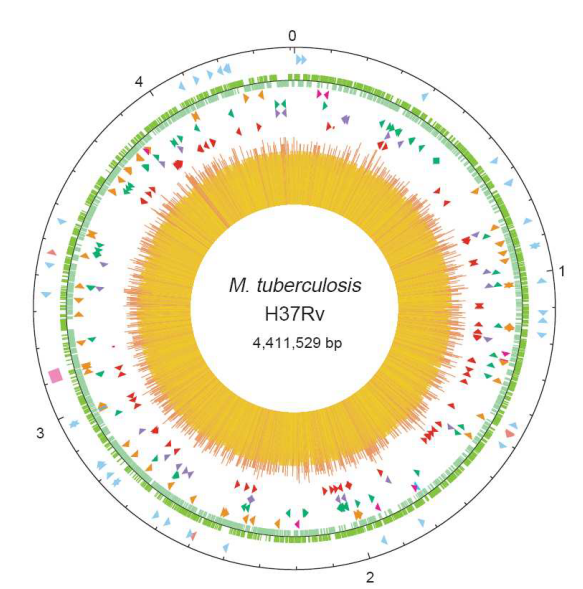
\includegraphics[width=0.9\linewidth]{genome.png}
    \end{center}
\caption[foo bar]{Круговая карта генома \ti{M. tuberculosis штамма} H37Rv.}
\label{genome}
\end{figure}

Следует отметить, что ключевые особенности организации генома одинаковы для всех штаммов патогена. Геномы представлены кольцевой молекулой ДНК протяженностью около 4400 тысяч пар оснований (т.п.о.) и характеризуются высоким содержанием GC пар (\~ 65.5\%). При этом существует несколько регионов, отличающихся по GC составу.

Углубленный анализ генома \ti{M. tuberculosis} штамма H37Rv выявил 3906 генов (аннотация RefSeq, \fl{NCBI Reference Sequence: NC\_000962.3}), кодирующих белки. При этом следует отметить, что альтернативный старт трансляции GTG встретился в 35\% случаев, что существенно чаще, чем 14\% и 9\% в геномах \ti{Bacillus subtilis} и \ti{Escherichia coli}, соответственно. Был найден один набор рибосомных генов и 45 транспортных РНК.

Первые результаты анализа геномных последовательностей \ti{M. tuberculosis} показали крайне малое разнообразие патогена на генетическом уровне по сравнению с другими видами бактерий. Дополнительно, методами популяционной генетики, была установлена крайняя степень клональности популяционной структуры \cite{sreevatsan1997restricted, ramaswamy1998molecular, hirsh2004stable}. Это обстоятельство в свое время наложило ограничение на использование метода мультилокусного типирования, столь широко применяемого для других бактериальных патогенов. Однако с развитием сравнительной геномики и усовершенствованием технологий полногеномного секвенирования на геномном уровне было найдено значительное количество вариаций, которые могут быть использованы для построения филогенетически надежных классификаций \cite{gagneux2007global}. Такими информативными маркерами для \ti{M. tuberculosis} послужили крупные делеции (large sequence polymorphisms, LSPs) и однонуклеотидные полиморфизмы (single nucleotide polymorphisms, SNPs). При этом важно подчеркнуть, что из-за достаточно малой вариации геномной последовательности патогена (штаммы в среднем отличаются друг от друга не более чем на 2,000 SNPs) вероятность возникновения независимой рекуррентной мутации крайне мала. Отсутствие горизонтального переноса генов дополнительно уменьшает возможность обратной мутации, а в случае с LSPs предотвращает появление геномных последовательностей, потерянных ранее. Основные работы, посвященные изучению популяционной структуры патогена, представлены на рисунке \ref{diser_pic_4}. Как видно из рисунка, в настоящее время выделяют 4 линии, относящиеся к \ti{M. tuberculosis}, и 2 линии, характеризующие \ti{M. africanum}.

\begin{figure}[h!]
    \begin{center}
        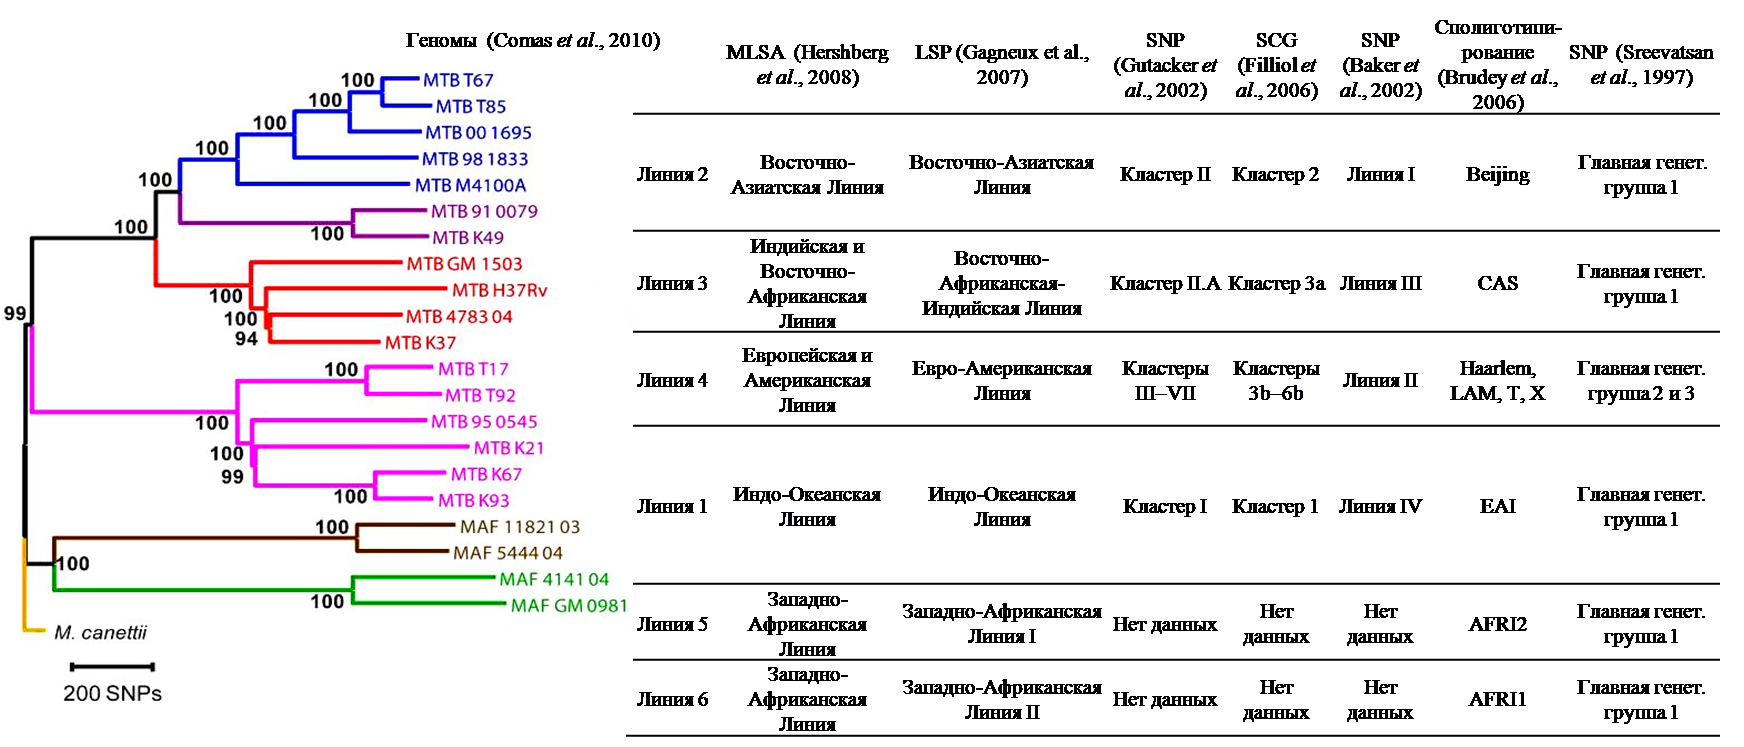
\includegraphics[width=0.9\linewidth]{diser_pic_4.png}
    \end{center}
\caption[foo bar]{Сравнение терминологии и молекулярных маркеров для определения основных линий внутри \ti{M. tuberculosis} и \ti{M. africanum}}
\label{diser_pic_4}
\end{figure}

\subsubsection{Генетическое семейство Beijing}
Впервые представители генотипа Beijing были обнаружены в 90х годах ХХ века, в двух независимых исследованиях, проведенных научными группами из Голландии и Америки \cite{van1995predominance, bifani1996origin}. В ходе IS6110 RFLP анализа и сполиготипирования коллекции изолятов \ti{M. tuberculosis}, полученных от больных ТБ в 1992-1994 годах в Китайской Народной Республике и Монголии, van Soolingen с соавт. выявили доминирующий генотип. При этом наиболее часто представители генотипа встречались в окрестностях Пекина (англ. Beijing), отчего и получили свое название \cite{van1995predominance}. Параллельно этому исследованию, Bifani с соавт. из Научно-исследовательского института общественного здравоохранения США (Public Health Research Institute, NY, США), в 1996 году методами молекулярно-генетической эпидемиологии описали вспышку лекарственно-устойчивого туберкулеза, произошедшую в Нью-Йорке в начале 1990х. Выявленные штаммы характеризовались крайне схожими паттернами IS6110 профилей и были названы «W» \cite{bifani1996origin}. В дальнейшем эти названия были объединены в W/Beijing или просто Beijing \cite{van2001molecular, kurepina1998characterization}. При этом название как нельзя лучше отражает реальное место зарождения генотипа. Его представители наиболее часто встречаются в Восточной Азии и, по мнению Мокроусова с соавт., генотип Beijing возник в Северном Китае более 1,000 лет назад. Дальнейшее его распространение было связано с миграционными потоками: со средневековых времен в Россию, совсем недавно в ЮАР (с XVII века) и в Австралию (в XIX веке) \cite{mokrousov2008molecular}. В свою очередь, согласно Merker с соавт., генотип в целом возник более 6,000 лет назад в географической зоне, включающей в себя Северо-Восток Китая, Корею и Японию \cite{merker2015evolutionary}.

Согласно международной базе данных сполиготипирования SpolDB4, штаммы Beijing присутствуют в наибольшем количестве стран на глобальном уровне (13\% от мирового количества изолятов), являясь по этому показателю уникальным генотипом \cite{brudey2006mycobacterium}. Здесь также следует отметить ассоциацию представителей генотипа с многочисленными вспышками заболеваний во всем мире, многие из которых были лекарственно устойчивые \cite{frieden1996multi, agerton1999spread, affolabi2009first, caminero2001epidemiological}. В структуре популяции возбудителя туберкулеза в России доля штаммов Beijing составляет от 50\% до 80\% \cite{mokrousov2003pcr}, причем, крайне выражена ассоциация штаммов с лекарственной устойчивостью \cite{casali2014evolution}. Исходя из сказанного выше, предполагается, что у штаммов данной эволюционной линии, возможно, развились уникальные свойства, которые позволили им распространиться по всему миру (клональная экспансия). По мнению многих авторов, этими свойствами являются: 1) способность «ускользать» от БЦЖ-вакцинирования 2) способность штаммов относительно быстро приобретать устойчивость к противотуберкулезным препаратам.

\subsubsection{Характеристика кластера Beijing В0/W148}
При описании генетического семейства Beijing необходимо учитывать, что это все-таки разнородная группа и даже внутри генотипа существуют более  «успешные» кластеры. Одним из таких кластеров является Beijing B0/W148. Впервые штаммы кластера были выявлены на рубеже ХХ и ХХI веков. В независимых исследованиях Нарвской, Курепиной и Portaels с использованием IS6110 RFLP типирования обнаружили группы кластеризующихся образцов, названные B0 (отечественная систематика) и W148 (иностранная систематика). Отличительной особенностью этих образцов было наличие двойной полосы (7.1 и 9.2 Kb) в верхней части профиля. В 2008 году штаммы Beijing B0/W148 с sensu stricto профилем и характерной двойной полосой были отнесены к Beijing B0/W148 \cite{mokrousov2008molecular}, а метод IS6110-RFLP типирования был признан «золотым стандартом» для выявления изолятов данной клональной группы. Дополнительными названиями кластера могут считаться CladeB \cite{casali2014evolution} и ECDC0002 (de Beer et al., 2014).

На сегодняшний день опубликовано достаточно много данных об ассоциации штаммов кластера с лекарственной устойчивостью, что является достаточным, для оценки степени опасности, исходящей от циркуляции изолятов B0/W148. Первая статья, описывающая российские штаммы \ti{M. tuberculosis}, выделенные в середине 1990-х, уже показала широкую распространенность МЛУ среди изолятов данного кластера \cite{marttila1998ser315thr}. Недавно изоляты B0/W148 с множественной лекарственной устойчивостью были выявлены в эпидемиологически значимой выборке пациентов с впервые выявленным ТБ в Ленинградской \cite{tratata123}, Тульской \cite{dubiley2010molecular}, Самарской и других областях. Следует отметить, что в исследовании более 1,000 штаммов из Самары 119 штаммов относилось к кластеру B0/W148 и все они были лекарственно устойчивы. В Абхазии, 22 из 23 изолятов В0/W148 были МЛУ, в то время как другие включенные в исследование изоляты генотипа Beijing были чувствительны к противотуберкулезным препаратам (10 из 55) \cite{pardini2009characteristics}. В Эстонии изоляты кластера B0/W148 составили 37.2\% от всех лекарственно устойчивых штаммов генотипа Beijing, в то время как ни одного чувствительного штамма B0/W148 в данном исследовании выявлено не было, включая штаммы, выделенные в 1994 году \cite{kruuner2001spread}. Также следует отметить, что в исследовании 2,092 образцов из 24 стран Европы методом VNTR кластер B0/W148 был выявлен в 470 случаях (17 стран, преимущественно Восточная Европа). Согласно исследованию этот кластер называется ECDC0002 и в крайней степени ассоциирован с лекарственной устойчивостью.
Довольно интересной является гипотеза о происхождении штаммов и первичном их распространении. По мнению Мокроусова штаммы кластера зародились в Сибири до 1960х годов, что в целом согласуется с исследованием Merker с соавт. (касательно даты возникновения). В дальнейшем, в ходе программы по освоению целины (1955-1960 годы), миграционные потоки были направлены в Казахстан и в Сибирь. Следует отметить, что в Казахстане представленность кластера В0/W148 крайне мала и составляет около 4\%. Это подтверждает гипотезу автора о том, что в европейской части России штаммов кластера в те годы еще не было. В свою очередь вторая волна миграции, 1960-1980 годы, напротив, из Сибири по всей стране могла повлечь массовое распространение представителей кластера. Согласно Мокроусову, триггером распространения именно устойчивого клона могло послужить повсеместное использование открытого в 1963 году рифампицина.
 
\subsection{Применение масс-спектрометрии в протеомике}
Протеомика исследует всю совокупность белков, синтезируемых организмом/клеткой в данной среде и на конкретном этапе клеточного цикла. Она описывает их качественный состав, относительную представленность, взаимодействие с другими макромолекулами, а также посттрансляционные модификации (ПТМ) \cite{haekkinen2000cell, molloy2002proteomics, monteoliva2004differential}. Белки играют важную роль почти во всех биологических процессах, соответственно в клетках существуют тысячи белков, каждый из которых подвергается взаимодействию, как с другими белками, так и с целыми клеточными компартментами.

Для исследования белков протеомика использует множество технических подходов. К ним относятся визуализация клеток с помощью световой и электронной микроскопии; эксперименты с кристаллами и изучением их структуры; и прочие. Другой мощный протеомный подход фокусируется на анализе \ti{de-novo} белков или совокупности белков, выделенных из клеток или тканей. Такие исследования, как правило, затруднительны из-за большой сложности клеточных протеомов и низкой представленности многих белков (а так же большого динамического диапазона концентраций белков), что требует высокочувствительных аналитических методов и приборов. Сейчас масс-спектрометрия (MS) становится основным методом для анализа сложных белковых образцов. Протеомика на основе MS - это дисциплина, основывающаяся на существовании баз данных последовательностей генов и геномов, а также техническим и концептуальным достижениям во многих областях, особенно, в создании и разработке методов ионизации \cite{aebersold2003mass}. За разработку методов идентификации и структурного анализа биологических макромолекул, и, в частности, за разработку методов масс-спектрометрического анализа биологических макромолекул, в 2002 году была вручена нобелевская премия Джону Фенну и Коити Танакака.

%\subsection{Проведение масс-спектрометрического эксперимента}
Стандартный эксперимент по исследованию белков с использованием масс-спектрометра состоит из пяти основных этапов. Схема представлена на рисунке \ref{mass_scheme}. На первом шаге белки из клеточного лизата или ткани извлекаются и очищаются. Как правило, за этим следует разделение полученной смеси гель-электрофорезом. Следующим этапом является фрагментирование белка на пептиды. Обычно это происходит при помощи фермента трипсина. На третьем этапе пептиды, предварительно разделенные жидкостной или иной хроматографией, подвергаются ионизации и поступают в масс анализатор. После MS-анализа пептиды могут подвергнуться повторной фрагментации. Новые, дочерние, ионы так же подвергаются анализу. Это пятый этап (MS/MS или тандемная масс-спектрометрия). МС-основанная протеомика зарекомендовала себя как незаменимая технология для определения закодированной в геноме информации. На сегодняшний момент белковый анализ (первичная структура, посттранскрипционные модификации или белок-белковые взаимодействия) при помощи МС является наиболее успешным при работе с небольшим (по сравнению с другими методами белкового анализа) количеством белка, выделенным из различных образцов. Системный анализ большого количества генов, экспрессированных в клетки, является основной целью протеомики; эта область сейчас быстро развивается, в основном, благодаря разработке новых экспериментальных подходов \cite{aebersold2003mass}.

\begin{figure}[ph!]
    \begin{center}
        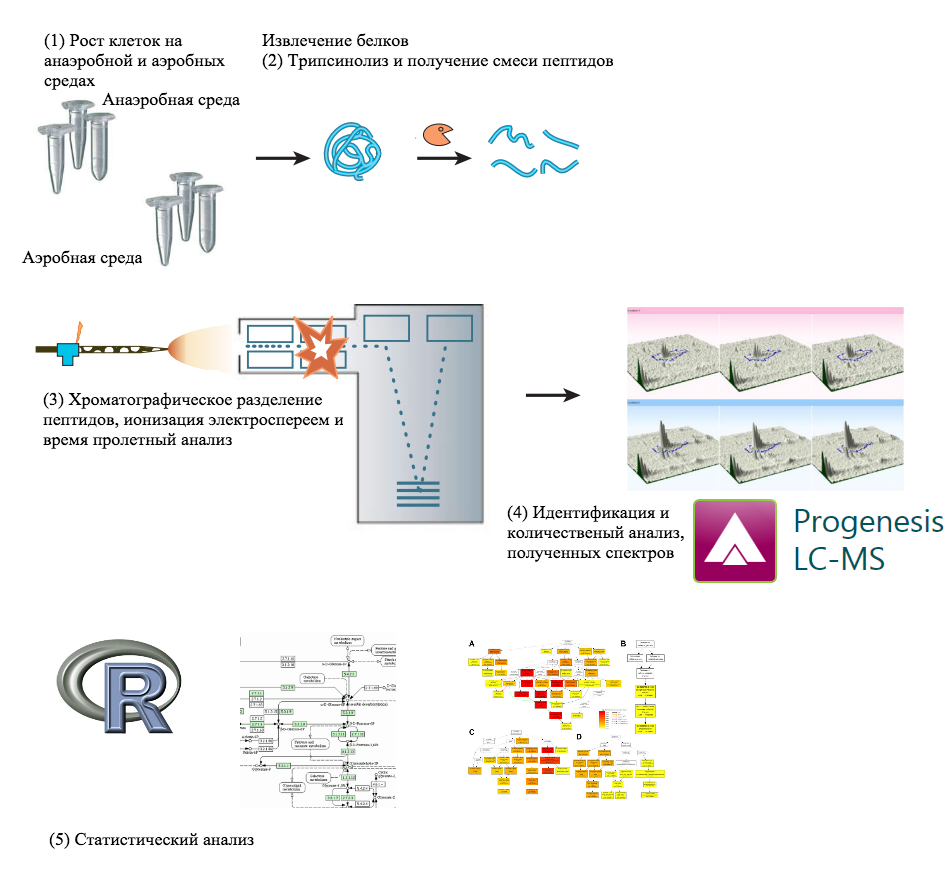
\includegraphics[width=0.9\linewidth]{mass_scheme.png}
    \end{center}
\caption[foo bar]{Схема проведения стандартного масс-спектрометрического эксперимента. Адаптировано из \cite{aebersold2003mass}.}
\label{mass_scheme}
\end{figure}

% \subsection{Orbitrap}

\subsection{Методы протеогеномики}
Для получения протеомных данных обычно используют метод <<\fl{shotgun proteomics}>> - комбинация жидкостной хроматографии и тандемной масс-спектрометрии \cite{bantscheff2012quantitative}. Одним из ключевых шагов в протеомике является идентификация пептидов на основе полученных MS/MS спектров. В отличие от геномных технологий, вроде ДНК или РНК секвенирования, где происходит непосредственное "прочитывание" исходной последовательности, в протеомике, как правило, пептиды идентифицируются за счет сопоставления экспериментальных MS/MS спектров и теоретических спектров всех пептидов, представленных в базе, против которой осуществляется поиск \cite{nesvizhskii2010survey}.
При таком поиске используются следующие исходные предположения: 
\begin{inparaenum}
    \item все белок-кодирующие последовательности генома точно известны и аннотированы
    \item все эти последовательности включены в базу, против которой осуществляется поиск
\end{inparaenum}.
Весь последующий анализ, включая идентификацию, количественный анализ и прочий статистический анализ, основывается на этих предположениях \cite{nesvizhskii2005interpretation}.

Проблема такого подхода заключается в том, что не все пептиды представлены в текущей поисковой базе или какой-либо другой. Пептиды могут содержать мутации, находиться в новых генах, перед неверно аннотированным стартом или в альтернативных сплайсформах. 
Один из способов идентификации пептидов с мутациями заключается в масс-тег подходе. При этом подходе происходит идентификация коротких участков пептида, после чего осуществляется поиск в более широком диапазоне масс прекурсеров \cite{dasari2010tagrecon}. 

Более общим подходом является протеогеномика. Термин впервые был использован в 2004 и изначально применялся в исследовании, где протеомные данные использовались для улучшения качества аннотации \cite{jaffe2004proteogenomic}. С тех пор этот термин используется в более общем смысле. В протеогеномном подходе, пептиды идентифицируются за счет идентификации MS/MS спектров против специальной базы, включающей в себя последовательности новых предсказанных белков, а так же различные варианты последовательностей уже аннотированных белков. Такие базы получаются за счет использования геномной и транскриптомной информации. Таким образом, протеогеномика позволяет не только подтвердить текущую аннотацию, но так же уточнить её \cite{nesvizhskii2014proteogenomics}. 

\subsubsection{Типы пептидов, идентифицируемых при протеогеномном исследовании}
Пептиды, идентифицируемые при протеогеномном поиске, соответствуют различным участкам генома. Такие пептиды можно разделить на межгенные (находятся между аннотированными генами) и внутригенные (находятся полностью или частично в областях, где содержится аннотированный ген). Внутригенные можно разделить на 
\begin{inparaenum}
    \item находящиеся в белок-кодирующих генах 
    \item находящиеся в длинных некодирующих РНК
    \item находящиеся в псевдогенах
\end{inparaenum} \cite{harrow2012gencode}. Большинство пептидов, идентифицируемых в протеогеномике, уже известны и относятся к аннотированным генам. В эукариотах (в которых присутствует интроно-экзоная структура) большинство пептидов относятся к экзомам, и, как правило, меньше 20\% относятся к экзон-экзон участкам. Новые пептиды, не идентифицируемые против какой-либо базы, могут находиться в неаннотированных участках генома, быть результатами единичной аминокислотной замены (SAP), находиться в нетранслируемых регионах (3' или 5' UTR) или интронах, являться результатом альтернативного сплайсинга \cite{nesvizhskii2014proteogenomics}.

\subsubsection{Подходы к созданию поисковых баз}
Идентификация пептидов против специальных баз является ключевым шагом в протеогеномике. Обычно база состоит из известных аннотированных и предсказанных последовательностей. При протеогеномном поиске следует внимательно относиться к размеру базы: увеличение размера влечет за собой увлечение времени поиска и FDR. Оптимальный выбор зависит от того, что требуется в эксперименте: точность или чувствительность \cite{nesvizhskii2014proteogenomics}. Рассмотрим наиболее распространенные варианты создания баз для протеогеномного поиска.

\textbf{Транслирование в шести рамках генома} - такая база может быть получена в результате транслирования в шести рамках генома \cite{baerenfaller2008genome}. Недостатком такого подхода является большой размер итоговой базы (в основном состоящей из последовательностей несуществующих белков) и невозможности поиска экзом-экзом пептидов, в случае эукариот. Например транслированный таким образом геном человека приводит к базе в ~3.2 гигабазы белковых последовательностей, что в 70 раз больше, чем референс в 45 мегабаз \cite{khatun2013whole}. Для уменьшения размера базы могут применены различные вычислительные методы: выбор последовательностей, имеющих гомологии с уже известными белками; использование методов предсказания кодирующего потенциала; исключение слишком коротких последовательностей (например, меньших, чем 30 аминокислот) \cite{blakeley2012addressing}. 

%\textbf{Ab initio предсказание генов} 

%\textbf{Expressed sequence tag (EST) data}

\textbf{Аннотированные РНК-транскрипты} Белковые последовательности могут быть получены в результате шестирамочного транслирования аннотированных РНК-транскриптов, например из баз Enselbl или RefSeq. Это позволяет идентифицировать альтернативные сайты инициации трансляции. База GENCODE содержит 84408 мРНК аннотированных белков. В результате транслирования такой базы получается белковая база в 200 мегабаз, что всего в 4.5 раза больше референса \cite{khatun2013whole}. Так же такие базы могут содержать последовательность, аннотированные как псевдогены или длинные некодирующие РНК \cite{derrien2012gencode}.

%\textbf{RNA-seq данные}

\textbf{Различные вариации последовательностей} Белковые последовательности в рефернсной базе могут быть дополнены последовательностями, являющимися вариациями референсных последовательностей (как правило, это SAP, делеции и инсерции). Для каждой вариации берется большая область вокруг неё и добавляется в базу, как отдельная, независимая последовательность. Одно аминокислотные замены можно скачать из различных баз данных: \fl{NCBI dbSNP, Online Mendelian Inheritance, Protein Mutant Database} \cite{li2011bioinformatics}.  

%\textbf{Прочие специализированные базы}

\subsubsection{Влияние размера базы}
Возможность идентифицировать спектры пептидов, полученные в результате MS/MS экспериментов, используя поисковые базы данных, зависит от многих факторов. Во-первых, пептид должен присутствовать в поисковой базе. Однако, чем больше сравнивается теоретических спектров с экспериментальным, тем больше вероятность того, что лучший результат будет у неверного теоретического спектра, и тем труднее различать верные и неверные идентификации \cite{nesvizhskii2010survey}. В результате, поиск против большой базы может дать несколько новых идентификаций белков или пептидов, но при этом общее количество идентификаций будет меньше, в сравнении с поиском против референсного сиквенса \cite{blakeley2012addressing, krug2013deep}. Так же увеличение базы приводит к увеличению машинного времени, необходимого для этого поиска. Таким образом, одним из ключевых моментов в протеогеномике является поиск баланса между размером базы и её содержимым.

\subsubsection{Способы увеличения чувствительности идентификации пептидов}
Протеогеномные базы, как правило, больше соответствующих белковых баз, используемых в обычных экспериментах. Чтобы компенсировать эту разницу можно применять различные методы и техники. Подходы, используемые в протеомике и протеогеномике для увеличения числа идентификаций, можно разделить на две группы: технические (связанные с подготовкой и непосредственно проведением масс-спектрометрического эксперимента) и вычислительные (связанные с различными подходами обрабоки и валидации полученных результатов). В качестве вычислительного подхода можно рассматривать идентификацию с помощью нескольких поисковых машин одного и того же набора данных \cite{shteynberg2013combining}. После поиска происходит изменение скорингов идентификации пептидов за счет комбинации нескольких источников информации, используя подходы машинного обучения \cite{nesvizhskii2010survey}. Например, такую функцию выполняет Scaffold, позволяющий объединить результаты поиска нескольких поисковых машин. Одной из дополнительных стратегий для сокращения пространства поиска является фракционирование смеси пептидов, проводимое до \fl{LS-MS/MS} анализа. Фракционирование, например, может проходить за счет определенных физико-химических свойств пептида или свойств последовательности пептида. Примером фракционирования может служить изоэлектрическая фокусировка. Спектры, полученные от фракции с определенной изоэлектрической точкой, можно искать против пептидов с примерно такой же теоретически предсказанной изоэлектрической точкой \cite{branca2014hirief}. Другим примером фракционирования может служить разделение геля на несколько полос, в результате чего происходит разделение исходной смеси пептидов. Независимое измерение каждой фракции позволяет снимать спектры низко-представленных пептидов, которые не были бы отобраны на MS-2, в случае, если бы фракционирование не проводилось \cite{bespyatykh2016proteome}.

Чувствительность идентификации так же можно повысить за счет многоступенчатого анализа данных. На первом этапе можно проводить поиск против \textquotedblleftэталонной\textquotedblright\ базы, наиболее точно описывающей исследуемый организм и позволяющей идентифицировать большинство спектров. На втором этапе происходит поиск против расширенной базы для идентификации дополнительных спектров \cite{ning2010computational, helmy2012mass}. При таком подходе результаты первоначального поиска используются для уточнения второй базы, используемой при дальнейшем анализе. 

\subsubsection{Точность идентификации}
Одной из целей протеогеномики является поиск новых областей генома, кодирующих белки, и уточнение уже аннотированных. Поэтому требуется дополнительная точность идентификаций, чтобы предотвратить внесение ошибок в аннотацию. Ошибки могут возникать и накапливаться практически на любом этапе работы. В протеогеномике, как и в протеомике, для предотвращения накопления ошибок при переходе с PSM на уровень уникальных пептидов, избыточные PSM должны быть свернуты в один PSM с наивысшим скорингом \cite{nesvizhskii2010survey}. Пептиды, идентифицированные в различных состояниях (например, двух- или трех-зарядные ионы; модифицированные и не модифицированные формы) так же должны быть объединены или обрабатываться вероятностно, с учетом удельных весов \cite{shteynberg2011iprophet}. 

При использовании многоэтапного поиска, когда результаты первой идентификации используются при подготовки базы для дальнейшей, более специфической идентификации, необходимо на каждом шагу добавлять соответствующие количество decoy-последовательностей в базу \cite{nesvizhskii2010survey}. 

Одним из способов отслеживания количества ложных идентификаций служит FDR, позволяющий оценить долю ложно-положительных идентификаций. Выделяют глобальный FDR, характеризующий общую долю ложно положительных идентификаций во всём эксперименте, и локальный, характеризующий вероятность ложной идентификации каждого отдельного пептида или белка. Кроме контроля глобального FDR, используемого в большинстве работ по протеомике, необходимо следить за достоверностью каждой отдельной идентификации (например, при глобальном пептидном FDR в 5\% ошибка идентификации отдельных пептидов может превышать это значение). Вероятность идентификации белка или события (новый ген, альтернативный старт, сплайс форма, в случае протеогеномики, может быть рассчитана на основании вероятностей соответствующих уникальных пептидов \cite{shteynberg2011iprophet, castellana2010proteogenomics}.

%\subsubsection{Класс-специфический анализ идентификаций и FDR}


\subsubsection{Ложная неслучайная идентификация пептидов}
Ошибочная идентификация пептида происходит в одном из двух случаев: либо произошло случайное совпадение с высоким скором MS/MS-спектра и несвязанного с ним пептидом из базы, либо в результате гомологии последовательности пептида из базы и истинной последовательности пептида. Вне зависимости от типа используемой при поиске decoy-базы (например реверсивное или случайное прочтение исходных последовательностей), ложные идентификации второго типа, скорей всего, будут недооценены \cite{nesvizhskii2010survey}. Часто ложная идентификация происходит в результате химической модификации высоко представленного пептида, если в результате сдвига масс из-за модификации, масса пептида становится эквивалента массе некоторого другого пептида из базы \cite{nesvizhskii2006dynamic, abraham2013moving}. Для исключения таких идентификаций можно проверить, например с использованием BLAST, схожесть последовательности каждого нового идентифицированного пептида, с последовательностями всех пептидов, представленных в референсной базе, и исключить (или отдельно контролировать) все высоко гомологичные. Если для дальнейшего анализа требуется сохранить такие пептиды (например при поиске одно аминокислотных замен), нужно проверить, что наблюдаемая разница масс между новым и референсынм пептидом не совпадает с массой какой-либо распространенной химической или пост-трансляционной модификацией \cite{li2011bioinformatics}. Список наиболее частных модификаций, специфичных для исследуемого биологического объекта, можно получить, используя 'blind' поисковый алгоритм \cite{tsur2005identification}. Кроме того, замена лейцина на изолейцин и обратная не может быть идентифицирована с помощью масс-спектрометрии. Пептиды, содержащие такие замены, должны быть исключены из дальнейшего анализа.

\subsubsection{Интерпретация данных и новых событий}
В протеомике результатом идентификации является список идентифицированных белков или генов, а так же список идентифицированных пептидов, с определенным уровнем FDR. В протеогеномике к таким результатам, так же добавляются списки новых событий, вроде "новый ген"\,, "новый кодирующий регион"\,, "альтернативный старт"\  и так далее, с соответствующими пептидами, подтверждающие эти события. Пептиды с одинаковыми последовательностями могут быть получены из различных областей генома (например, от паралогов, идентичных сайтов разных белков или из псевдогенов). Такие пептиды не могут быть доказательством экспрессии с какого-то определенного участка генома \cite{nesvizhskii2005interpretation}. Кроме того, новые пептиды могут быть интерпретированы разными способами, например как новый транскрипт этого гена или как пептид из интрона или нетранслируемого региона того же гена. 

\subsubsection{Идентификация новых пептидов}
Одним из результатов протеогеномного анализа является список новых пептидов. Этот список зависит от выбора референсной базы и её версии. Как обсуждалось ранее, для многих организмов существуют несколько версий белковых баз, и эти базы отличаются объемом и качественном аннотации. Более того, эти базы регулярно обновляются, в результате в них добавляются и удаляются последовательности. Таким образом, в протеогеномным исследованиях, пептиды идентифицируемые против специфичных баз, должны быть проверены на вхождение в основанные базы, существующие для данного организма.

\subsection{Применение протеогеномики}

\subsubsection{Поиск новых белок-кодирующих регионов}
Возможность применение масс-спектрометрических протеомных данных для поиска новых белок-кодирующих регионов и подтверждения границ уже аннотированных, обсуждалась начиная с первых дней существования протеомики, как науки в её современном виде \cite{choudhary2001interrogating, andersen2001mass}. Такие результаты чаще всего достигаются за счет поиска против специальных баз данных, полученных в результате шести рамочного транслирования генома, трех рамочного транслирования предсказанных различными методами белок-кодирующих участков генома или шести (трех, в случае стрнед-специфичного секвенирования) рамочного транслирования данных РНК-секвенирования. Как правило, новые белок-кодирующие регионы находят у новых, немодельных организмов \cite{castellana2014automated, castellana2008discovery, yang2011discovery}. Даже для хорошо исследованых эукариот есть работы, в которых находят новые гены. Например, исследование белкового профиля человека и мыши с использованием шестирамочного транслирования, позволило идентифицировать 98 и 52, соответственно, ранее не аннотированных белок-кодирующих областей \cite{branca2014hirief}.

\subsection{Идентификация коротких рамок считывания и сайтов инициации трансляции}
Предсказание коротких рамок считывания (sORF) и рамок, начинающихся не с канонических старт-кодонов, особенно затруднительно \cite{yang2011discovery}. В работе Yang и соавторов было показано, что короткие рамки могут составлять до 10\% от всех белок-кодирующих элементов в геноме эукариот \cite{yang2011discovery}. Хотя с развитием методов рибопрофилирования и РНК-секвенирования появилась возможность находить sORF, протеогеномика позволяет получить дополнительное подтверждение белок-кодирующего потенциала этих sORF \cite{menschaert2013deep, oyama2007diversity, slavoff2013peptidomic}. Поиск пептидов, подтверждающих sORF и сайты инициации трансляции, будет более эффективным, если провести дополнительные этапы подготовки образца. Для повышения вероятности идентификации белков из sOFR можно использовать фракционирование, перед LC-MS/MS экспериментом \cite{slavoff2013peptidomic}. Для обнаружения новых сайтов инициации трансляции, как правило, требуется точная идентификация N-концевого пептида, которые могут быть обогащены перед масс-спектрометрическим анализом за счет использования N-концевых меток \cite{hartmann2014n}. 


\subsection{Протеогеномика \ti{M. tuberculosis}}
\subsubsection{\ti{M. tuberculosis} H37Rv}
Для проверки и корректировки аннотации Kelkar и соавторы провели протеогеномное исследование \ti{M.tuberculosis} H37Rv с использованием масс-спектрометрических данных \cite{kelkar2011proteogenomic}. В своей работе, в качестве геномной базы, авторы использовали транслированный в шести рамках геном. В качестве стартовых кодонов использовались GTG и TTG, которые транслируются как метионин, а не валин и лейцин соответственно, в случае, если они являются стартовыми сайтами \cite{cole1998erratum}. 

GSSP пептиды были разделены на 3 группы:
\begin{inparaenum}
    \item относящиеся к межгенным областям
    \item частично пересекающиеся с аннотированным геномом
    \item полностью относящиеся к аннотированным генам
\end{inparaenum}.

Они обнаружили 41 новый ген, и корректировку рамки для 79 генов. Из 79 генов с измененной рамкой: для 78 было исправлено положение стартового кодона, и два гена были объединены в один. Для подтверждения этих результатов использовались альтернативные программы для аннотации генома (\fl{FgeneSB, GeneMark 2.5}), а так же поиск гомологий среди известных генов, используя алгоритм BLAST. 

Авторы работы были удивлены, что они обнаружили новые гены с учетом того, что геном был секвенирован более 10 лет назад, и аннотирован множеством независимых групп.

\subsubsection{\ti{Mycobacterium smegmatis}}
Похожее исследование было проведено Potgieter и соавторами для \ti{Mycobacterium smegmatis}. В своей работе они использовали две геномные базы: одну для поиска новых генов, другую для идентификации TSS. 

Первая база была получена в результате транслирования в шести рамках геном бактерии. В качестве стартовых кодонов использовались ATG, GTG, и TTG. Исключались последовательности, длина которых была меньще 20 аминокислот. В результате получилась база в 79481 последовательностей. При поиске против этой базы было идентифицированною 77 ORF, не содержащих аннотированных генов, по 1 пептиду, и 44 ORF по двум и более пептидам. Для ORF, идентифицированных только по одному пептиду была проведена дополнительная проверка: выполнялось выравнивание с использованием BLAST против известных протеомных и транскриптомных баз. В результате 19 ORF были отобраны, как "низкоуровневые доказательства"\ для изменения аннотации генома.

Вторая база использовалась для поиска TSS. Она была получена в результате \ti{ab inito} предсказания белок-кодирующих генов, с использованием программы GeneMarkS. Так же эта база подтверждала новые гены и изменения в уже аннотированных. Размер базы составил 6655 последовательностей. При поиске против этой базы было идентифицировано 137 не триптических TSS-пептидов и 547 триптических TSS-пептидов. Так же было идентифицировано 3 ORF с альтернативными сайтами начала трансляции \cite{potgieter2016proteogenomic}. 



\newpage

\section{Материалы и методы}

\subsection{Получение бактерий}

\subsection{Проведение масс-спектрометрического эксперимента}

\subsection{Контроль качества}

\subsection{Идентификация}

\subsection{Коилчественный анализ}
\subsubsection{Анализ в MaxQuant}
\subsubsection{Анализ в Progenesis LC-MS}
\subsubsection{Сравнение результатов программ}

\subsection{Протегеномика}

\newpage

\section{Результаты и обсуждение}

\subsection{Подготовка и проведение масс-спектрометрических измерений}
Тут что-нибудь про бактерий напиать.
Были отсняты масс-спектры 30 культур. Из них 6 были не фракционированы, остальные были разделены на 6 фракций. Разделение на фракции позволило идентифицировать пептиды, которые не были бы идентифицированы при обычном поиске, из-за того, что на измерения MS/MS спектра были бы отобраны более высоко представленные пептиды. Количество отснятых спектров для каждой культуры представлены в таблице.

\subsection{Подготовка баз}
Скаченная с NCBI аннотация содержала 4103 аннотированных белок-кодирующих последовательностей. После добавления контаминант и decoy-последовательностей получилась белковая база, состоящая из 8258 последовательностей. После транслирования генома в 6 рамках и исключения коротких последовательностей получилось 74488 белок-кодирующих последовательностей. В результате добавления контаминант и decoy-последовательностей, получилась геномная база, состоящая из 149028 последовательностей. Исключение коротких последовательностей из геномной базы позволило ускорить поиск; снизить пороговые значения идентификации, тем самым повысив чувствительность подхода. Минимальная длинна аннотированного белка \ti{W-148} составляет 84 аминокислоты, таким образом, исключение рамок длинной меньше чем 33 аминокислоты не должно привести к потерям при идентификации.

\subsection{Идентификация белков и пептидов}
Поиск проходил при помощи поисковых маших Mascot и X!Tandem. Объединение результатов поиска и перерасчет FDR был произведен в Scaffold. Против белковой базы было идентифицировано 32054 пептида (1041059 psm), против геномной базы 36502 уникальных пептида (1131085 psm). Пересечение идентифицированных пептидов представлено на рисунке \ref{Identification}. Часть пептидов идентифицирована против белковой базы и не идентифицирована против более полной полной геномной базы. Это связано с различными пороговыми скорингами при поиске против баз разных размеров. 
После вычитания результатов поиска против белковой базы из результатов поиска против геномной базы получилось 6015 GSSP (Genome search specific peptides).  После исключения пептидов представленных в аннотированном геноме и идентифицированных только против геномной базы, осталось 1397 GSSP. Наличие таких пептидов, идентифицируемых только против геномной базы и представленных в аннотации, связано с пересчетом FDR: при отдельном рассмотрении результатов идентификации каждой поисковой машины таких эффектов не возникает.  После исключения GSSP, представленных только в одной культуре, осталось 425 пептидов. Результаты интерпретации GSSP при таких фильтрах: 16 новый ORF, и 304 гена с корректированным положением старта.  
Пептидов, интерпретируемых как пептиды перед аннотированным стартом примерно в 8 раз больше, чем пептидов, относящихся к новым генам. Такой разброс может быть связан с тем, что пептидам относящимся к корректировке рамки проще пройти порог FDR. В самом деле, при пептидном и белковом FDR в 1\% и, примерно, 1000000 psm при размере базы в 4000 аминокислотных последовательностей, 10000 пептидов будут ложно-положительно идентифицированы. Если брать критерий 2 и более пептидов для идентификации белка, то такого количества пептидов будет достаточно для идентификации 5000 белков, если не учитывать белковой FDR. С учетом белкового FDR количество ложно-положительно идентифицированных белков должно быть не боле 40. Для этого достаточно 80 пептидов. Таким образом, в экспериментах с большим количеством исходных данных, белковый FDR становится более жестким критерием, чем пептидный. Соответственно, GSSP относящимся к корректировке рамки проще пройти белковый FDR, так как в этой рамке так же присутствуют пептиды из аннотированной части последовательности. В случае нового гена в "прохождение"\ белкового FDR участвуют только GSSP пептиды.

\begin{figure}[pH]
    \begin{center}
        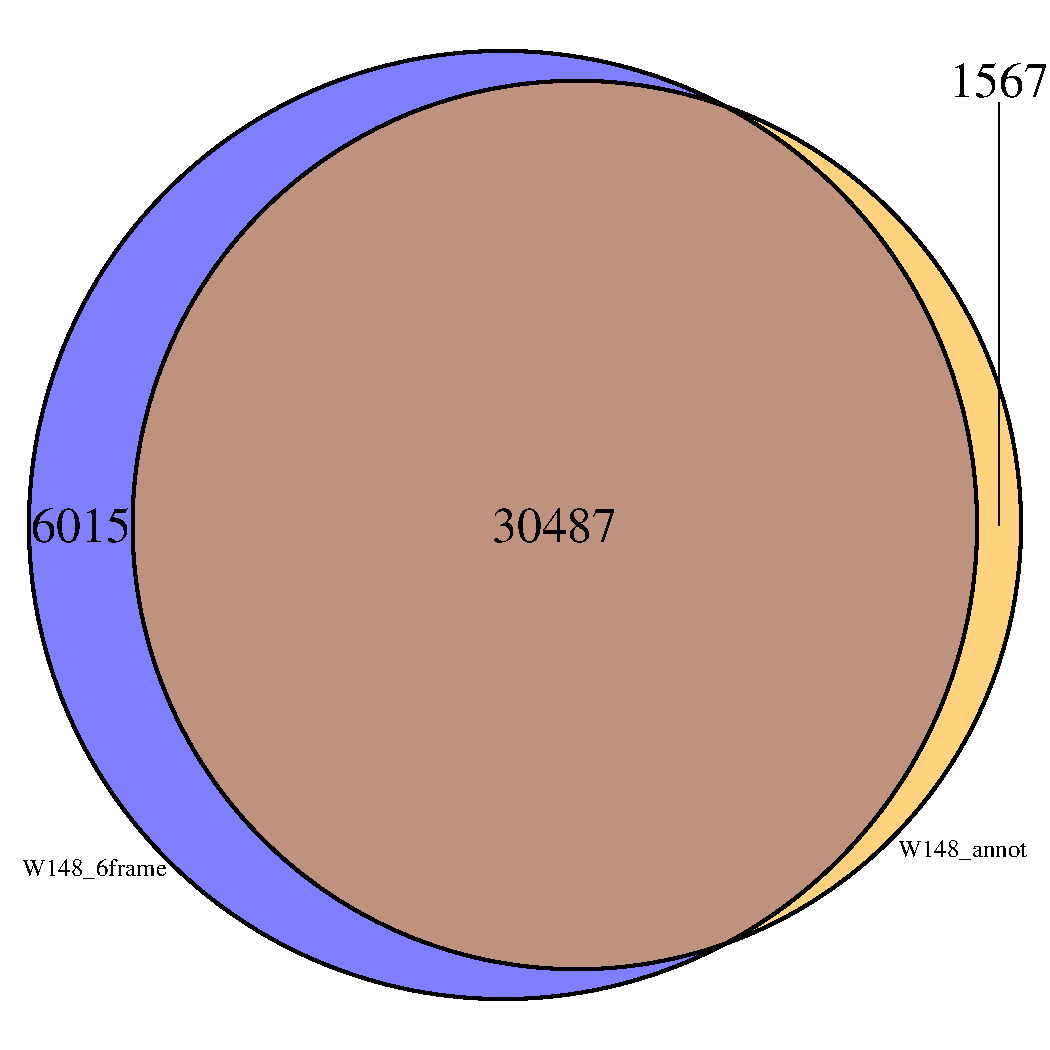
\includegraphics[width=0.9\linewidth]{Identification.pdf}
    \end{center}
\caption[foo bar]{Сравнение идентификаций против различных баз:
  \begin{enumerate*}%[label=\textit{\alph*)}]
    \item annot - количество уникальных пептидов идетифицированных против белковой базы
    \item 6frame - количество уникальных пептидов идетифицированных против геномной базы
  \end{enumerate*}.}
\label{Identification}
\end{figure}

Для подтверждения результатов были применены дополнительные критерии. После удаления PSM, ошибка идентификации которых составляет более трех стандартных отклонений в предположении о нормальном распределении ошибки идентификации всех PSM в интервале +/- 5 минут, остался 331 уникальный GSSP. Следует отметить, что на этом шаге отсекались пептиды, ошибка идентификации которых меньше, чем реальная точность приборов. Поэтому данный критерий отнесен к дополнительным. Затем была проведена фильтрация по времени выхода. После исключения 10\% наиболее отклоняющихся пептидов, остался 147 уникальный GSSP. 

Все GSSP были проверены на точное вхождение в базу NCBInr. Среди белков, в которых нашлись GSSP, не было найдено  таких, которые бы относились к организмам, которые ранее снимались на используемом масс-спектрометре. Таким образом можно исключить остаточную контаминацию на приборе и пробоподготовке. Так же были исключены 8 пептидов, которые присутствуют в аннотированных последовательность \ti{W-148} с учетом одной замены.

\subsection{Интерпретация новых событий}
\subsubsection{Новые ORF}
Было идентифицировано 16 новых ORF, в которых присутствует 2 и более уникальных GSSP. Из шестнадцати ORF пять пересекаются с аннотированными псевдогенами, одиннадцать лежат на комплиментарной цепи участков с аннотированными генами. У пяти из шестнадцати есть гомолог в \ti{H37Rv}. Гены всех \ti{M.tuberculosis} плотно расположены, и межгенные области либо отсутствуют, либо их длинна намного меньше длины гена, либо, если межгенник большой, в нем находится псевдолен. Поэтому не найдено новых генов, которые не относились бы к псевдогенам и лежали в межгенном пространстве.

Следует отметить, что причины по которым ген становится "псевдоегном"\ с точки зрения биологии и системы аннотации NCBI различны. Так, наиболее частыми причинами из-за которых участок генома аннотируется как псевдоген являются: фреймшифт (потеря или вставка не кратного трем числа нуклеотидов, в результате чего нарушается белковая последовательность), неполный ген (присутвствует только часть гена, в сравнении с гамологами), стоп-кодон по середине последовательности, низкое качество сборки (например, если ген находится на стыке контигов). Для всех идентифицированных псевдогенов была найдена "техническая"\ и "биологическая"\ причина, из-за которой они получили статус псевдогена. Пример идентифицированно псевдогена представлен на рисунке \ref{pseudo_1}.

\begin{figure}[ph!]
    \begin{center}
        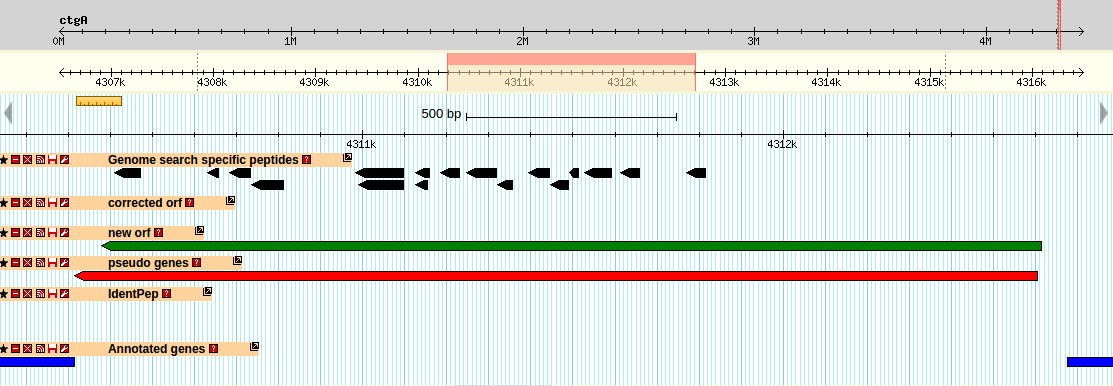
\includegraphics[width=1.2\linewidth, angle=-90]{pseudo_1.png}
    \end{center}
\caption[foo bar]{Идентифицированный псевдоген. Сними обозначены аннотированые гены, красным - псевдоген, зеленым - открытая рамка считывания, Genome search specific peptides - пептиды, идентифицируемы только про поиски против геномной базы}
\label{pseudo_1}
\end{figure}

\begin{figure}[ph!]
    \begin{center}
        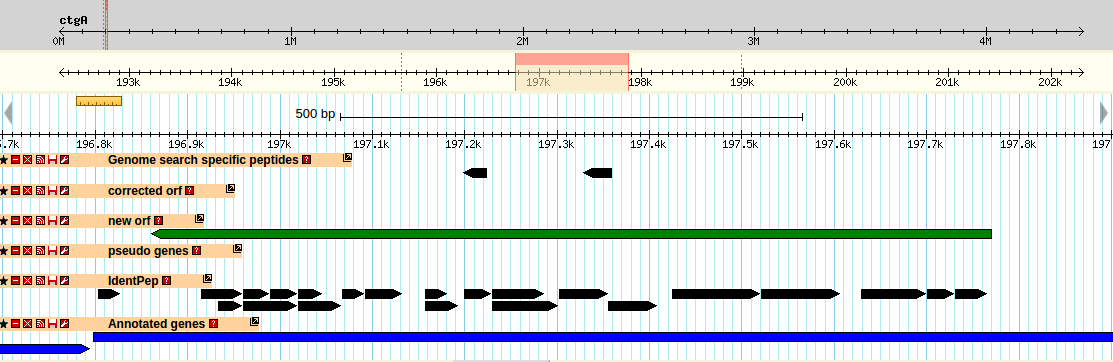
\includegraphics[width=1.2\linewidth, angle=-90]{comp_gene.png}
    \end{center}
\caption[foo bar]{ORF, лежащий на комплиментраной цепи к аннотированому и экспрессирующемуся гену. Сними обозначены аннотированые гены, IdentPep - идентифицрованные при поиске против белковой базы пептиды, красным - псевдоген, зеленым - открытая рамка считывания, Genome search specific peptides - пептиды, идентифицируемы только про поиски против геномной базы}
\label{comp_gene}
\end{figure}

\begin{figure}[ph!]
    \begin{center}
        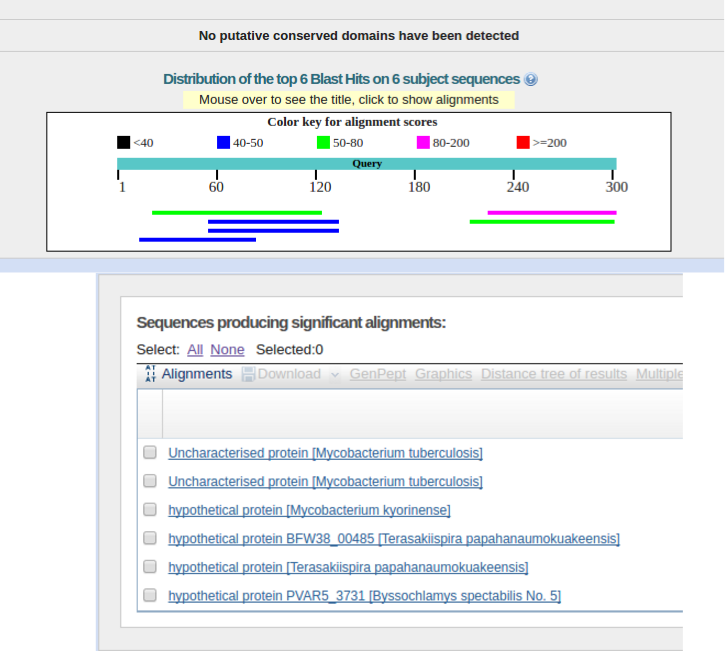
\includegraphics[width=1\linewidth]{comp_gene_blast.png}
    \end{center}
\caption[foo bar]{Результат поиска гомолога ORF, лежащей на комплиментарной цепи и предсталвенной на рисунке \ref{comp_gene}) против базы NCBInr с ипользованием алгоритма blast.}
\label{comp_gene_blast}
\end{figure}


В результате поиска против базы NCBInr при помощи алгоритма blust для десяти из одинналцати ORF, лежащих на комплиментарной цепи (пример такого ORF предствлен на рисунке \ref{comp_gene}) к аннотированным генам, были найдены гомологи. Эти гомологи были аннотированы как “гипотетический/предсказанный/непроверенный белок” другого штамма \ti{M.tuberculosis}. Косвенно результаты идентификации подтверждает тот факт, что все новые ORF лежат на комплиментарной цепи, а не в другом фрейме аннотированной. В самом деле, с пространственной точки зрения предположение, что транскрипт снимается с комплиментарной цепи выглядит более вероятным, чем предположение, что с одного транскрипта идет трансляция в двух фреймах двух разных аминокислотных последовательностей.

После применения дополнительных критериев фильтрации GSSP осталось шесть ORF с псевдогенами и один ORF на комплиментарной цепи.

\subsubsection{Корректировка положения аннотированного старта}
Всего 304 рамки содержат аннотированный ген и GSSP пептид. Из 304 308 содержат два и более GSSP. Эти рамки сравниили с гомологичными генами в \ti{H37Rv}. Из 38 36 совпадают с точностью до SAP, 2 рамки длинней у \ti{W-148}, чем у \ti{H37Rv}. Для этих 38 рамок были проверены пептиды, пересекающиеся аннотированный старт. Для 17 из 38 были найдены пептиды, содержащие в себе аннотированный старт (overlap-пептиды), для 7 были найдены стартовые пептиды из аннотации, для 3 были найдены как стартовые, так и аннотированные пептиды.

\subsubsection{Пептиды, содержащие аннотированный старт}
Для 17 из 38 рамок, содержащих аннотированный ген и два более GSSP, были найдены пептиды, содержащие в себе стартовую аминокислоту для аннотированного гена. Такой пептид представлен на рисунке \ref{overlap_pep}. Для 7 из 38 были найдены пептиды, являющиеся стартовыми для аннотированного гена. У 3 из 38 найдены как стартовые, так и overlap-пептиды, причем в этом месте не было сайта трипсинолиза.

\begin{figure}[h!]
    \begin{center}
        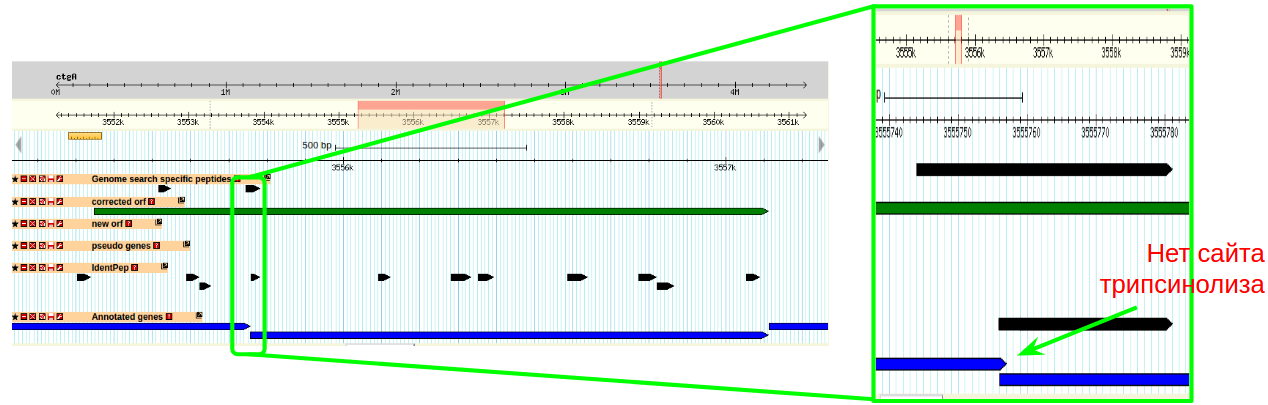
\includegraphics[width=1\linewidth]{overlap_pep.png}
    \end{center}
\caption[foo bar]{Ген с измененой рамкой считывания. Черным обозначены идентифицированные пептиды. Верхний глиф - GSSP, нижний - пептиды, идентифицированные при поиске против белковой базы. Идентифицирован как стартовый пептиы, так и overlap-пептид. Сайта трипсинолиза в этом месте нет. }
\label{overlap_pep}
\end{figure}



\newpage



































\newpage

\section{Выводы}

\begin{enumerate} 
\item Применение нескольких поисковых машин, с последующим объединением результатов, позволяет увеличить количество и качество идентификаций.

\item При обработке большого количества данных использование белкового FDR позволяет сократить количество ложно-положительные идентификаций белков, так как этот критерий становится более весомым, чем пептидный.

\item В результате протеогеномного анализа штамма \ti{Mycobacterium tuberculosis} W-148 были идентифицированы 16 новых генов и у 249 (24) открытых рамок считывания были скорректированы старты трансляции.

\item Разработано программное решение для протеогеномного анализа, которое можно за короткое время перенести на любой прокариотический организм.
\end{enumerate}
\newpage

\bibliographystyle{gost705}
\bibliography{bibliography}
\end{document}

% рекомендуется оформлять текст шрифтом Times New Roman от 12 до 14 pt
% межстрочный интервал 1.5
% выравнивание в абзацах по ширине
% поля на странице: левое – 30 мм, остальные 20 мм.



